\section{Resolución Problema 5}
\subsection{Problema:}
Dado un numero binario de $n$ bits regresar su equivalente en decimal.

\subsection{\textbf{Descripción del problema:}}

El reporte analiza el concepto de ingresar un número de tipo binario con $n$ bits, para posteriormente regresar su equivalente en decimal.

\begin{figure}[h!]
    \centering
    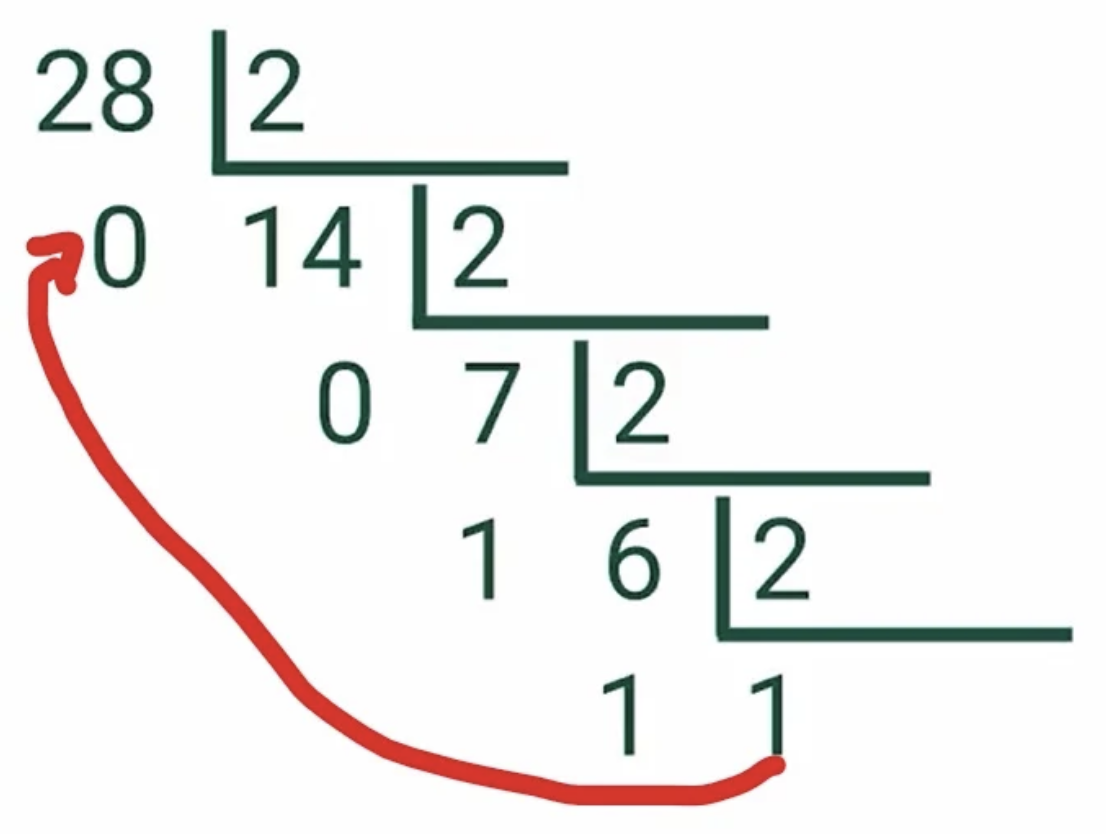
\includegraphics[width = 6 cm]{./latex-imágenes/conversionbin5.png}
    \caption{Conversión de binario a su equivalente decimal}
    \label{fig:GraficaEcuacionRecta}
\end{figure}

\subsection{\textbf{Definición de solución:}}

Los números binarios se conforman con los símbolos 0 y 1, que se combinan para representar cualquier número. 
Para representar números superiores a 1 dígito, se aplica un método semejante al de formación de números decimales, combinando ordenadamente los símbolos. Se repiten las combinaciones de dígitos anteriores y se le añade un dígito para continuar la numeración

\begin{table}[h]
     \centering
     \caption{Valores binarios}
     
     \begin{tabular}{|c|c|}
     \hline
        Corrida & Binario \\
        \hline
        0  & 0 \\
        \hline
        1  & 1 \\
        \hline
        2  & 10 \\
        \hline
        3  & 11 \\
        \hline
        4  & 100 \\
        \hline
        5  & 101 \\
        \hline
        6  & 110 \\
        \hline
        7  & 111 \\
        \hline
        8  & 1000 \\
        \hline
        9  & 1001 \\
        \hline
        10  & 1010 \\
        \hline
        11  & 1011 \\
        \hline
        12  & 1100 \\
        \hline
     \end{tabular}
     \label{tab:my_label}
 \end{table}

En el sistema binario se utiliza la ponderación por posición de dígito en la misma forma que en la numeración decimal, por ejemplo:

\begin{table}[h!]
     \centering
     \caption{Ponderaciones}
     
     \begin{tabular}{|c|c|c|c|c|}
     \hline
        Posición & 3 & 2 & 1 & 0 \\
        \hline
        ponderacion  & 2^{3} & 2^{2} & 2^{1} & 2^{0} \\
        \hline
        Peso en decimal  & 8 & 4 & 2 & 1 \\
        \hline
        Número en binario  & 0 & 1 & 0 & 1 \\
        \hline
     \end{tabular}
     \label{tab:my_label}
 \end{table}

El resultado da la operación se obtiene de hacer la operación “res=0*8+1*4+0*2+1*1”

\subsection{\textbf{Diseño de la solución:}}

\begin{figure}[h!]
    \centering
    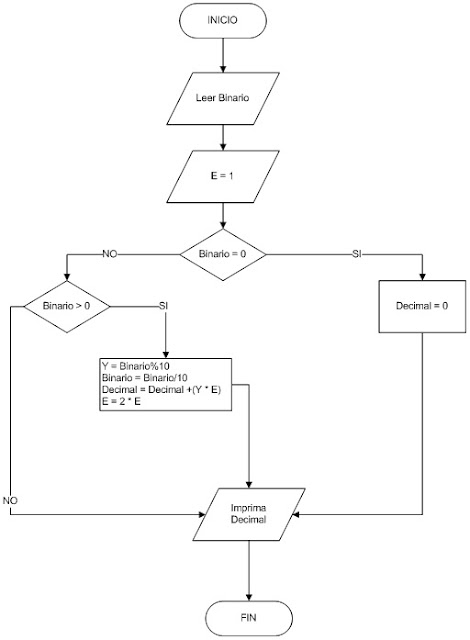
\includegraphics[width = 6 cm]{./latex-imágenes/dflujo5.jpg}
    \caption{Diagrama de flujo de el algoritmo de solución}
    \label{}
\end{figure}

\begin{enumerate}
    \item Solicitar al usuario que ingrese el número binario de n bits.
    \item Validar que el número binario ingresado sea válido, es decir, que esté compuesto únicamente de 0's y 1's y tenga una longitud de n bits.
    \item Calcular el número decimal equivalente utilizando el método binAdecimal.
    \item Mostrar el resultado al usuario.
\end{enumerate}

\subsection{\textbf{Desarrollo de la solución:}}

El algoritmo de solución del problema comienza solicitando al usuario teclee el número binario a convertir, para posteriormente almacenarlo en la variable $nbinario$.
\begin{javaCode}

Scanner in = new Scanner(System.in);
        
    System.out.println("ALGORITMO PARA CONVERTIR UN NÚMERO BINARIO A DECIMAL");
    System.out.println("------------------------------------------------------------------------");
    System.out.println("Ingresa el número binario correspondiente: ");
    String nbinario = in.nextLine();
    in.close();
        
\end{javaCode}

Se inicializa un $if$, esto con la finalidad de que si se llega a ingresar el signo "-", la conversión lo elimine.

\begin{javaCode}

if (nbinario.contains("-")) {
    nbinario = nbinario.replace("-", "");
    }

\end{javaCode}

Posteriormente, se vuelve a inicializar un $if$, este para realizar la operación de conversión únicamente si el dato de entrada contiene 0 y 1, de lo contrario, cancelar la conversión arrojando un mensaje de error.

\begin{javaCode}

if (nbinario.matches("[01]+")) {
    int num = binAdecimal(nbinario);
    System.out.println("Número decimal: " + num);
    }else{
        System.out.println("Carácter de tipo inválido");
    }
\end{javaCode}

Si la condición anterior se cumple, se manda a llamar al método $binAdecimal$, que es el que contiene todo el proceso de conversión.
\begin{javaCode}

public static int binAdecimal(String binario) {
    int n = binario.length();
    int decimal = 0;
       
    for (int i = 0; i < n; i++) {
        int bit = Character.getNumericValue(binario.charAt(i));
    decimal += bit * Math.pow(2, n - 1 - i);
    }

    return decimal;
}
    
\end{javaCode}

\subsection{\textbf{Depuración y pruebas:}}

\begin{table}[h!]
     \centering
     \caption{Tabla de Corridas}\\
     
     \begin{tabular}{|c|c|c|}
     \hline
        Corrida & Binario & Decimal\\
        \hline
        1  & 010111 & 23\\
        \hline
        2  & 011011 & 27\\
        \hline
        3  & 101010 & 42\\
        \hline
        4  & 010101 & 21\\
        \hline
        5  & 111011 & 59\\
        \hline
     \end{tabular}
     \label{tab:my_label}
 \end{table}
\vspace*{-8pt}